En esta sección se definen los casos de uso del sistema, los cuales describen las interacciones entre los actores y la aplicación para cumplir los requerimientos funcionales de la sección anterior. Para facilitar su lectura, los casos de uso se organizaron por módulos funcionales, cada uno representado mediante un diagrama de casos de uso de UML.

En la Figura~\ref{fig:casouso1} se presentan los casos de uso del módulo de autenticación y cuenta, que comprende el registro, la verificación del correo, el inicio y cierre de sesión, y la gestión de la contraseña y de la cuenta. En la Figura~\ref{fig:casouso2} se muestran los del módulo de perfil y ayuda, y en la Figura~\ref{fig:casouso3} los del módulo de lugares favoritos.

Los casos de uso del módulo de mapas y selección de ubicaciones se presentan en la Figura~\ref{fig:casouso4}, mientras que en la Figura~\ref{fig:casouso5} se generan los correspondientes al cálculo y selección de rutas. Por su parte, la Figura~\ref{fig:casouso6} muestra los casos de uso de la navegación activa, y la Figura~\ref{fig:casouso7} los del módulo de seguimiento, que abarca la creación y administración de enlaces y códigos de seguimiento, así como la consulta de la ubicación de las personas seguidas.

\begin{figure}[H]
    \centering
    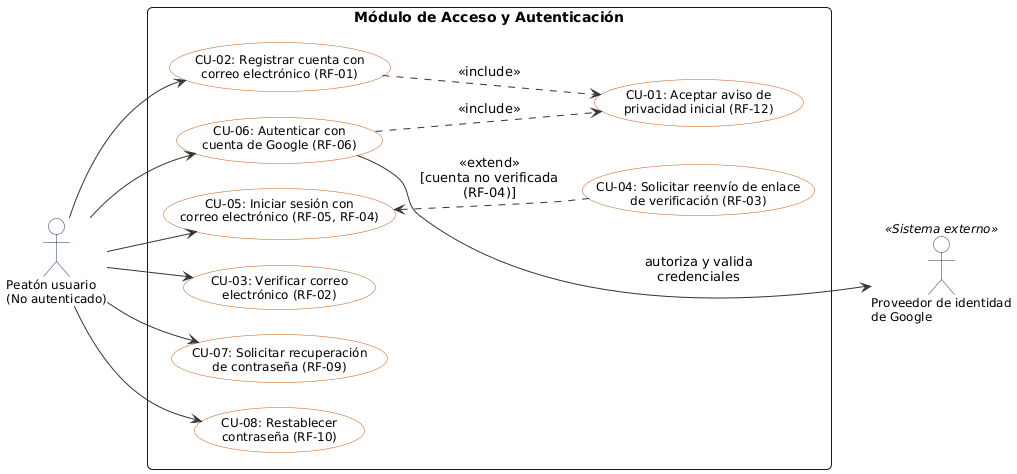
\includegraphics[width=1.0\linewidth]{figures/capitulo6_diseno_sistema/6.2_Casos_de_uso/1.png}
    \caption{Diagrama de caso de uso de módulo de autenticación y cuenta}
    \label{fig:casouso1}
\end{figure}

\begin{figure}[H]
    \centering
    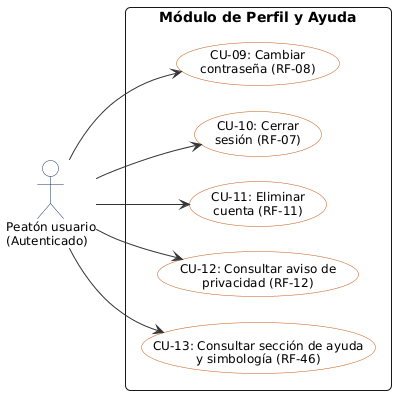
\includegraphics[width=0.7\linewidth]{figures/capitulo6_diseno_sistema/6.2_Casos_de_uso/2.png}
    \caption{Diagrama de caso de uso de módulo de perfil y ayuda}
    \label{fig:casouso2}
\end{figure}


\begin{figure}[H]
    \centering
    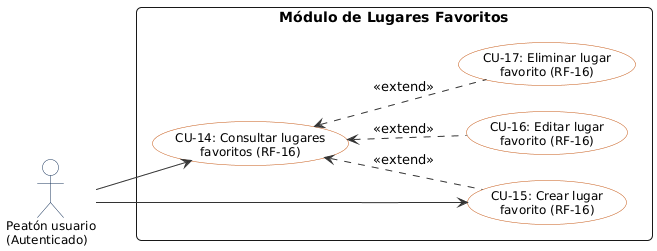
\includegraphics[width=1.0\linewidth]{figures/capitulo6_diseno_sistema/6.2_Casos_de_uso/3.png}
    \caption{Diagrama de caso de uso de módulo de lugares favoritos}
    \label{fig:casouso3}
\end{figure}


\begin{figure}[H]
    \centering
    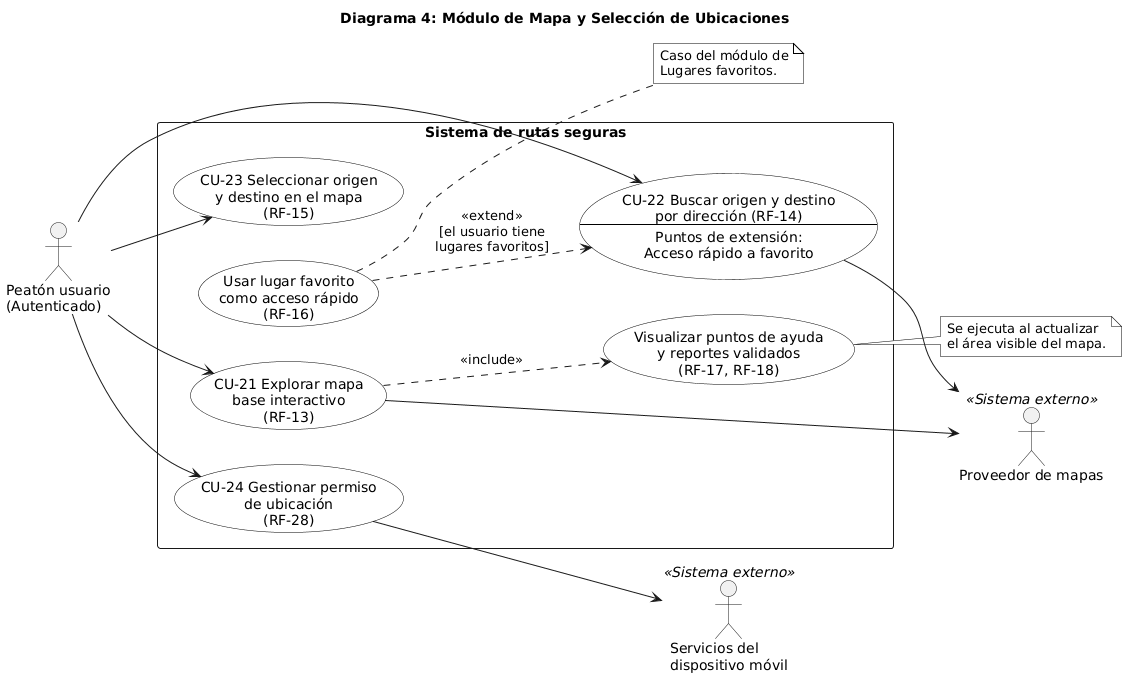
\includegraphics[width=1.0\linewidth]{figures/capitulo6_diseno_sistema/6.2_Casos_de_uso/4.png}
    \caption{Diagrama de caso de uso del módulo de mapas y selección de ubicaciones}
    \label{fig:casouso4}
\end{figure}


\begin{figure}[H]
    \centering
    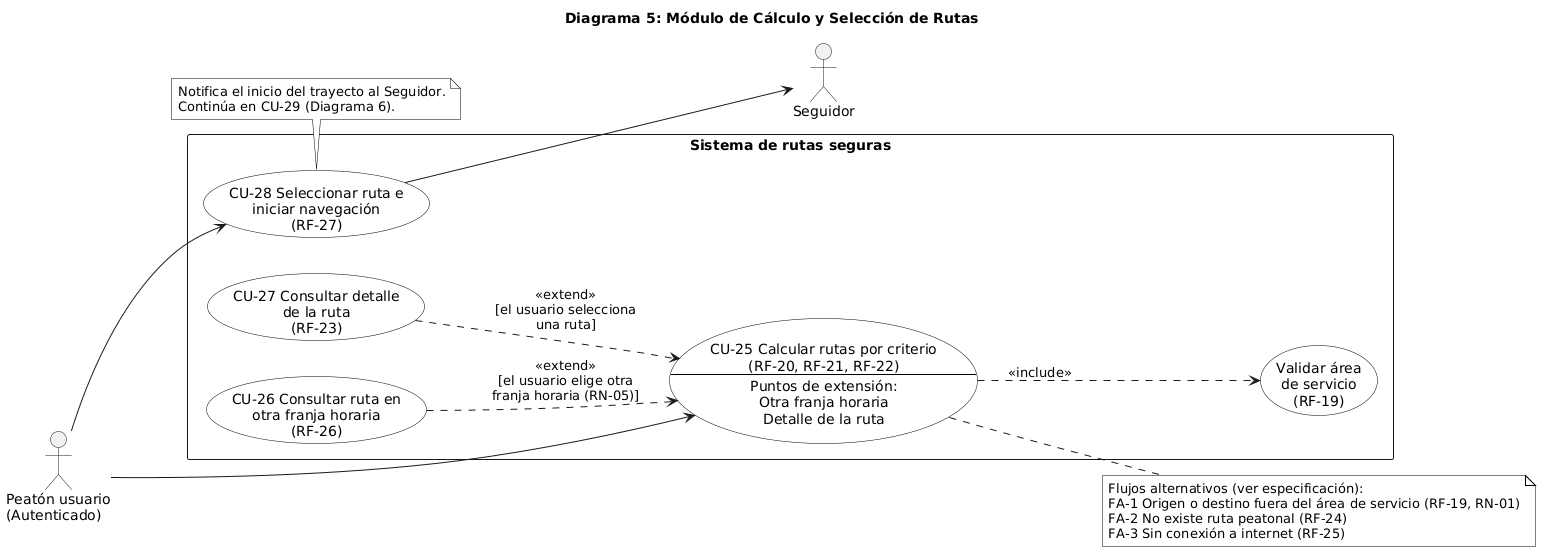
\includegraphics[width=1.0\linewidth]{figures/capitulo6_diseno_sistema/6.2_Casos_de_uso/5.png}
    \caption{Diagrama de caso de uso del módulo cálculo y selección de rutas}
    \label{fig:casouso5}
\end{figure}


\begin{figure}[H]
    \centering
    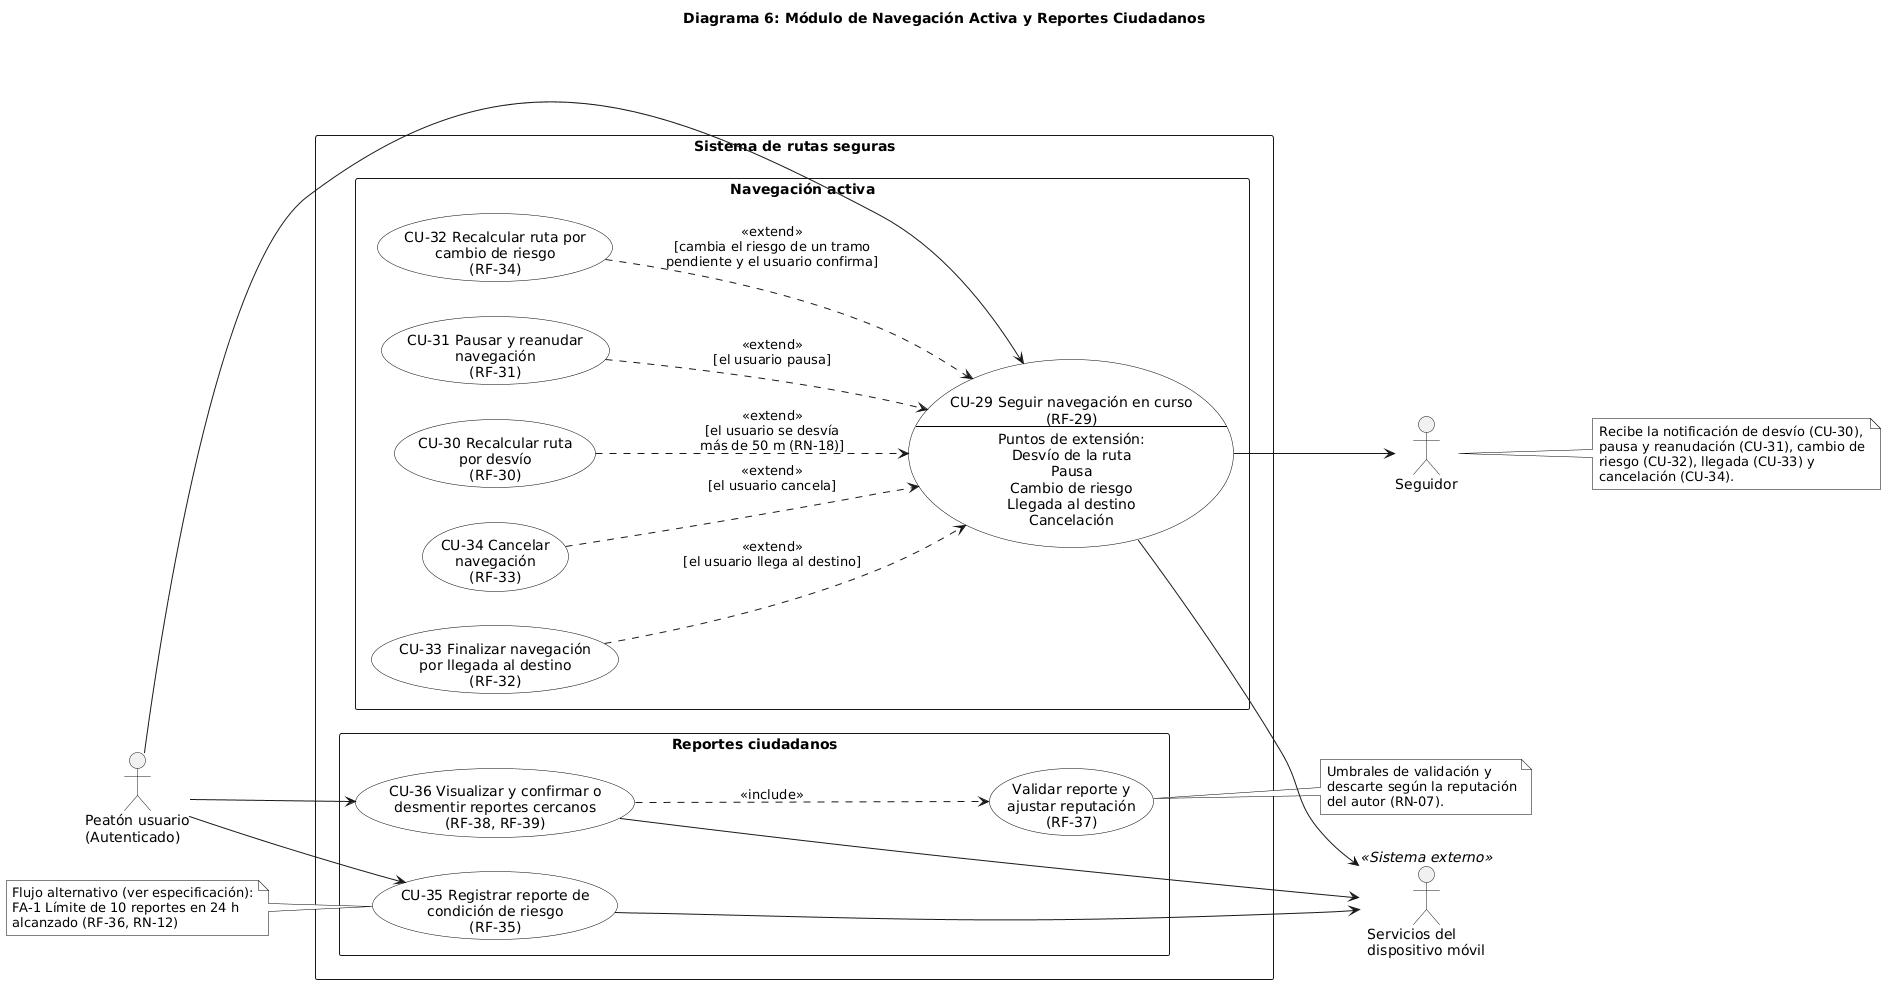
\includegraphics[width=1.0\linewidth]{figures/capitulo6_diseno_sistema/6.2_Casos_de_uso/6.png}
    \caption{Diagrama de caso de uso del módulo de navegación activa}
    \label{fig:casouso6}
\end{figure}


\begin{figure}[H]
    \centering
    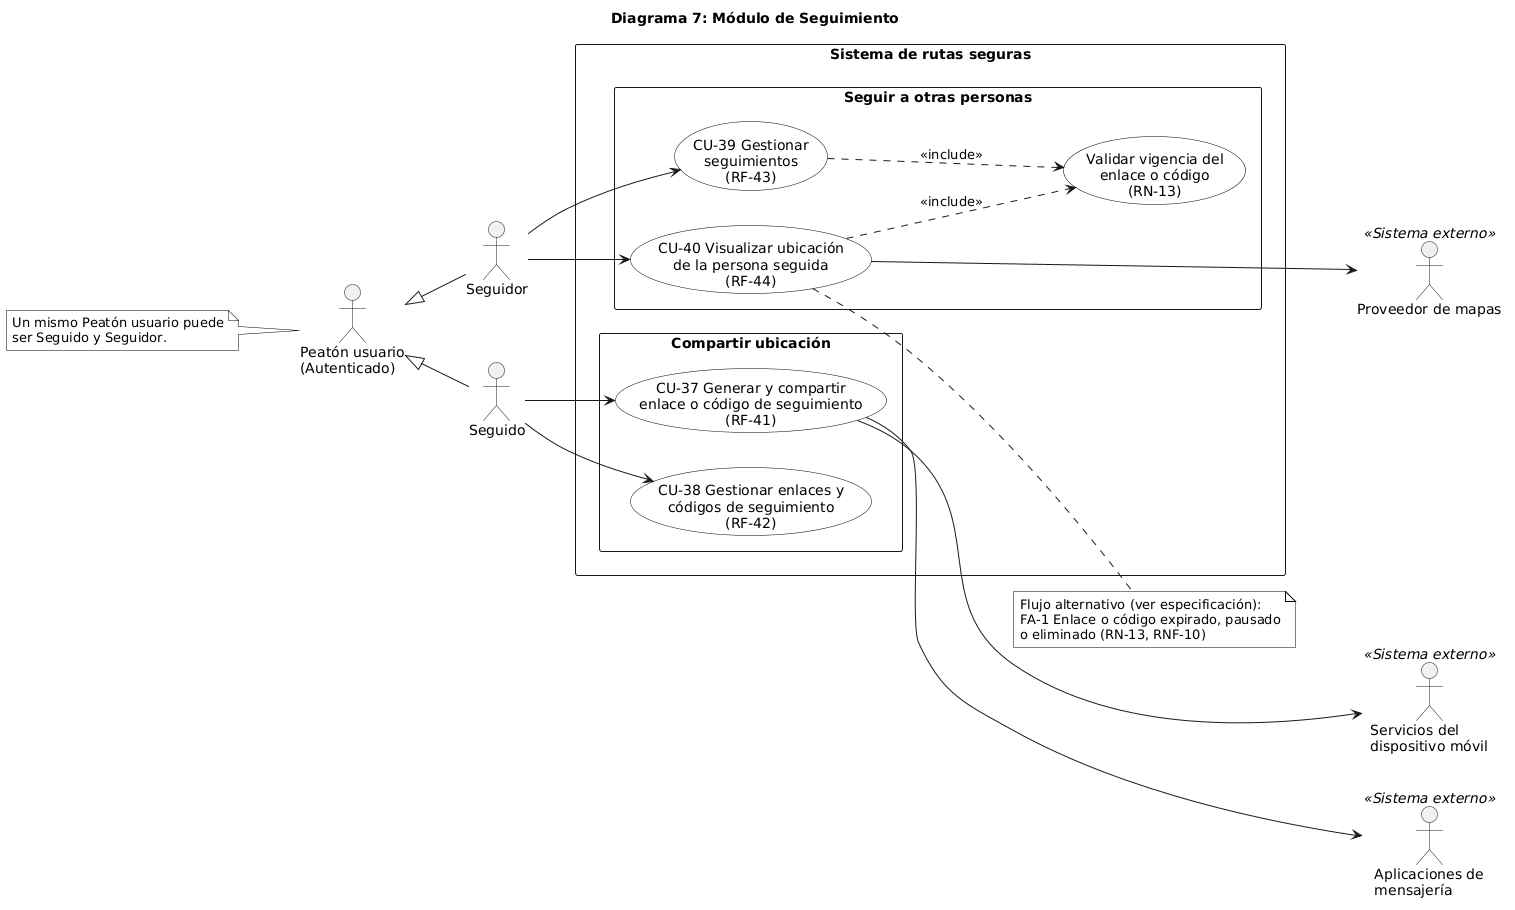
\includegraphics[width=1.0\linewidth]{figures/capitulo6_diseno_sistema/6.2_Casos_de_uso/7.png}
    \caption{Diagrama de caso de uso del módulo de seguimiento}
    \label{fig:casouso7}
\end{figure}
